\subsubsection*{Binning Methods}
\addcontentsline{toc}{subsubsection}{Binning Methods}%

Alternative binning methods for the production events underlie the developed hypothesis of this thesis work: Non-random features of the association networks derived from these two methods explained in the introduction part.

Two distinguished network generation approach can be derived considering the alternative binning tools mentioned above: Fixed Step Size network (FSSn); it has graph nodes as binning members with equal bin sizes, and Fixed Bucket Size network (FBSn); its nodes are binning members with an equal amount of events per bin. Forcing events to occur in the nodes with constant interval boundaries allows us to see how the aggregations take place within orders, whereas defining a typical bucket size for the network nodes results in arbitrary interval boundaries for each node; still, it allows to control their population.

%say that the event groups with the lower \& upper bounds (the so-called bin size): $700$-$799$ and $800$-$899$ can be produced together or the ones with the bounds: $500$-$599$ and $600$-$699$ likely occur in the identical sequences. It is also possible to investigate the relations between different bins (event groups) with equal event counts per bin among the complete data set.

%It is also possible to investigate the relations between different bins (event groups) with equal event counts per bin among the complete data set.
 \begin{figure}[!ht]
	\begin{center}
		\makebox[\textwidth]{
			\centering
			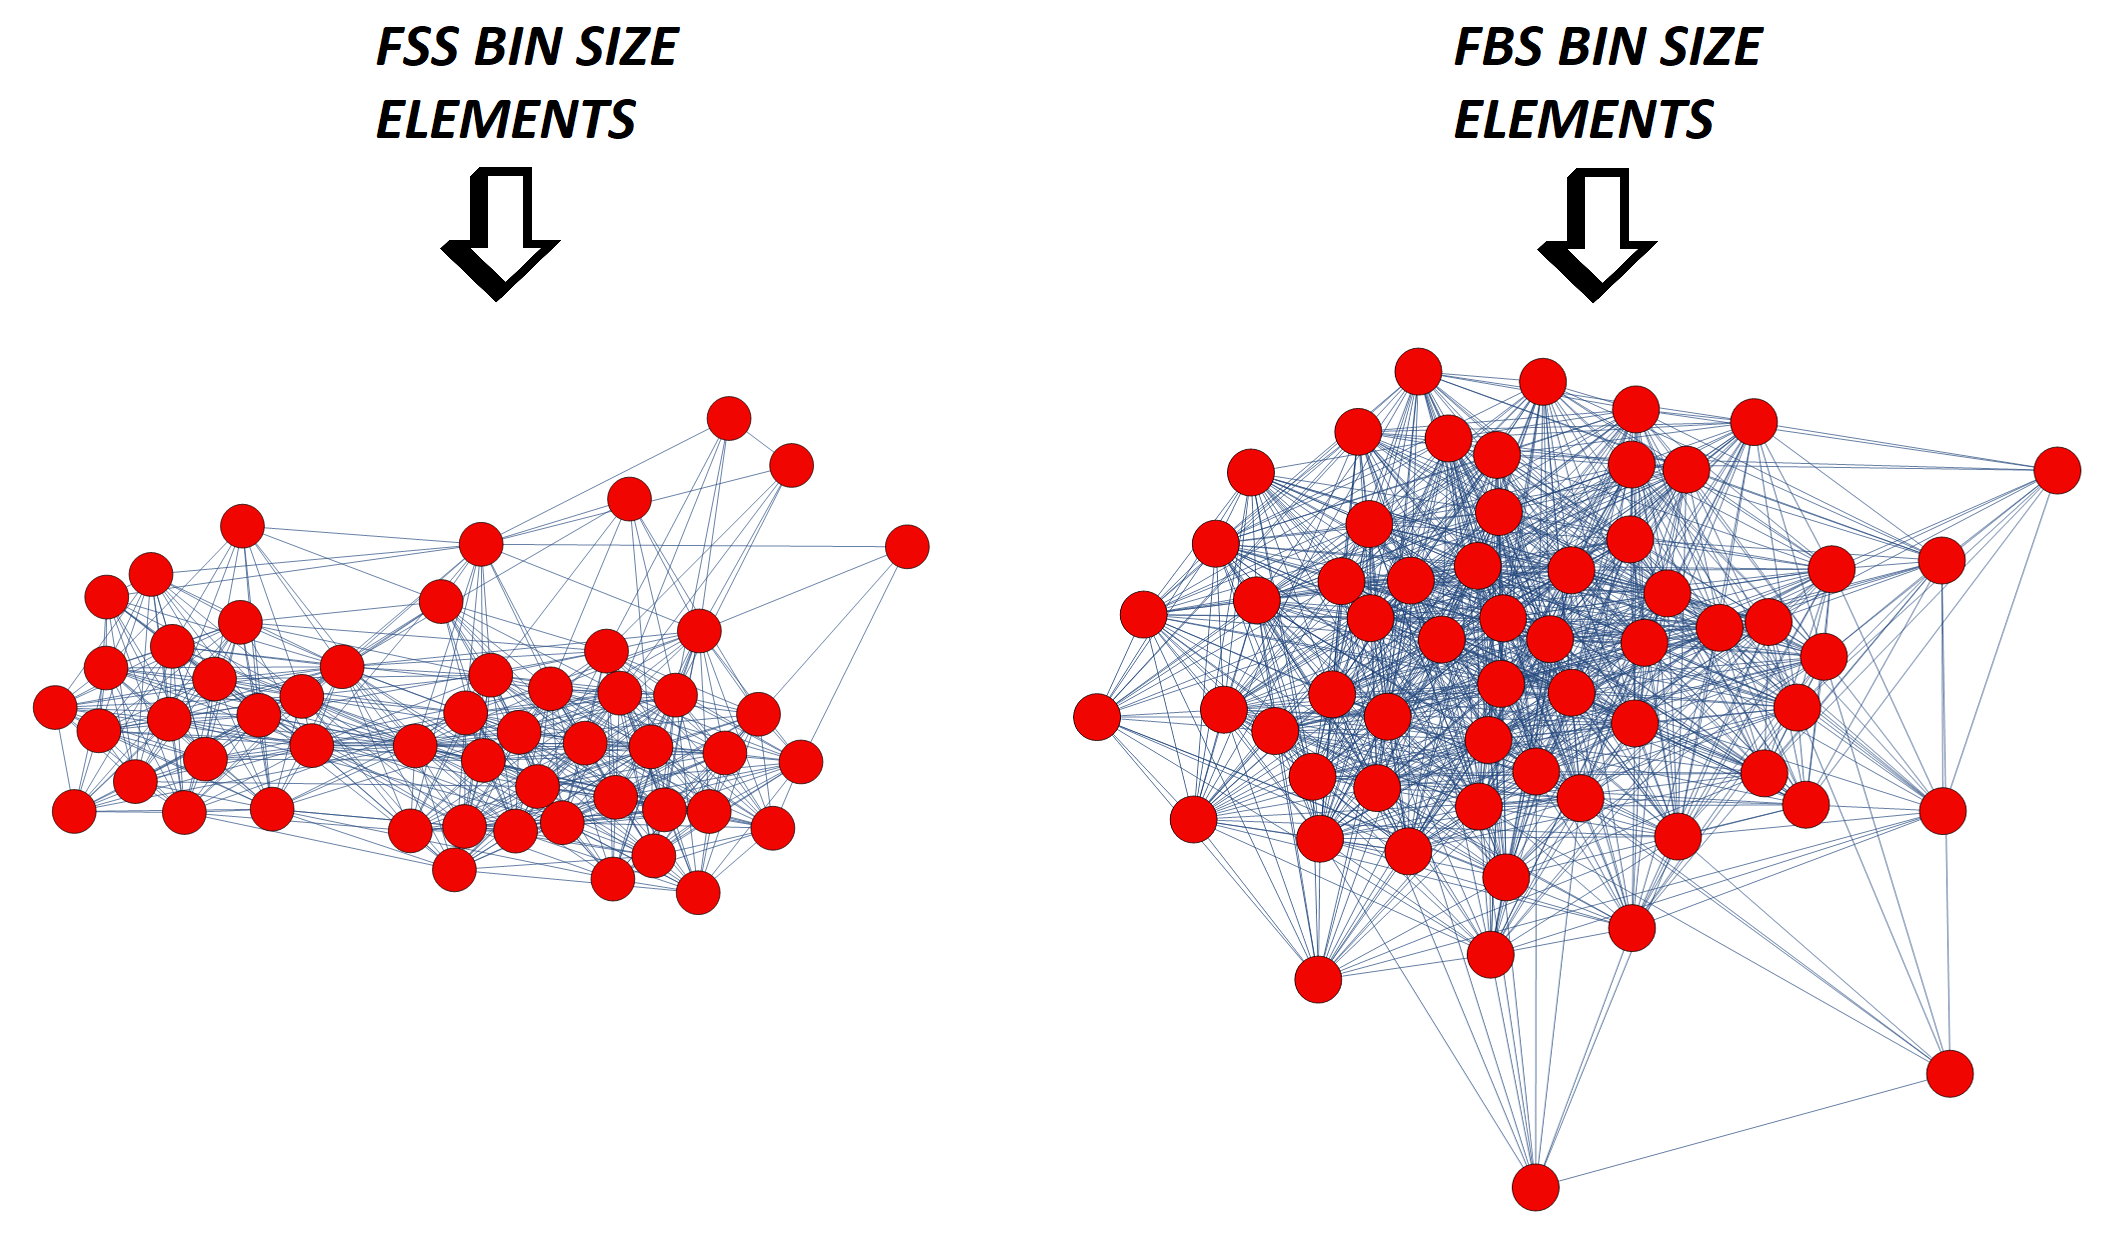
\includegraphics[width=0.8\linewidth]{../images/methodology-association-networks-hyp_networks.png}}
		\caption{Graph Results For Two Different Network Approaches.}
		\label{figure-hyp_graphs}
	\end{center}
\end{figure}
\clearpage

%\begin{table}[hb!]
%	\centering
%	\caption*{$D$ Labeled with FSS Bin Sizes}
%	\begin{tabular}{|ccccccc|l}
%		\cline{1-7}
%		\makecell{Event\\ID} 	&& Mass    	&& \makecell{FSS\\Bin Size}&& \makecell{Sequence\\ID} &  \\ \cline{1-7}
%		1 	      && 280	    && 200-299	&& 1 		   &  \\
%		2 		  && 250	    && 200-299	&& 1 		   &  \\
%		3 	      && 890	    && 800-899	&& 2 		   &  \\
%		4 		  && 850	    && 800-899	&& 2 		   &  \\
%		\vdots	  && \vdots  	&& \vdots	&& \vdots 	   &  \\
%		n-2 	  && 520	    && 500-599	&& k 		   &  \\
%		n-1       && 630	    && 600-699	&& k 		   &  \\
%		n 		  && 610	    && 600-699	&& k 		   &  \\ \cline{1-7}
%	\end{tabular}
%	\label{Tab:D-dataset-FSS}
%\end{table}
%\begin{table}[hb!]
%	\centering
%	\caption*{$D$ Labeled with FBS Bin Sizes}
%	\begin{tabular}{|ccccccc|l}
%		\cline{1-7}
%		\makecell{Event\\ID} 	&& Mass    	&& \makecell{FBS\\Bin Size}&& \makecell{Sequence\\ID} &  \\ \cline{1-7}
%		1 	      && 280	    && 200-599	&& 1 		   &  \\
%		2 		  && 250	    && 200-599	&& 1 		   &  \\
%		3 	      && 890	    && 630-899	&& 2 		   &  \\
%		4 		  && 850	    && 630-899	&& 2 		   &  \\
%		\vdots	  && \vdots  	&& \vdots	&& \vdots 	   &  \\
%		n-2 	  && 520	    && 200-599	&& k 		   &  \\
%		n-1       && 630	    && 630-899	&& k 		   &  \\
%		n 		  && 610	    && 600-629	&& k 		   &  \\ \cline{1-7}
%	\end{tabular}
%	\label{Tab:D-dataset-FBS}
%\end{table}